\documentclass[11pt,a4paper]{article}

\usepackage[utf8]{inputenc}
\usepackage[T1]{fontenc}
\usepackage[french]{babel}
\usepackage[margin=2.3cm]{geometry}
\usepackage{amsmath,amssymb}
\usepackage{graphicx}
\usepackage{booktabs}
\usepackage{tabularx}
\newcolumntype{C}{>{\centering\arraybackslash}X}
\usepackage{subcaption}
\usepackage{enumitem}
\usepackage[hidelinks]{hyperref}

\graphicspath{{figures/}}
\setlist{itemsep=2pt,topsep=4pt}

\title{Projet SDP -- Jalon 2\\[2pt]\large Apprentissage de deux modèles MR-Sort sur une clientèle segmentée (inv-2-MR-Sort)}
\author{Mohamed Salh \and Mohamed Chebli \and Quentin Robidou}
\date{Octobre 2026}

\begin{document}
\maketitle

% =====================================================================
\section{Problème}

Chaque objet $x=(x_1,\dots,x_n)$ du learning set est affecté à l'une de $p$ catégories ordonnées. On fait
l'hypothèse que ces affectations proviennent de \emph{deux} segments de clientèle, chacun décrit par son propre
modèle MR-Sort (profils $b^1,\dots,b^{p-1}$, poids $w$, seuil $\lambda$), mais on ne sait pas à quel segment
appartient chaque objet. Il faut donc, simultanément, partitionner le learning set en deux et apprendre un
modèle MR-Sort par partie. Apprendre un seul MR-Sort étant déjà NP-difficile, nous proposons une heuristique
qui s'appuie sur la bibliothèque \texttt{lincs} pour apprendre chaque modèle.

% =====================================================================
\section{Méthode d'apprentissage}

\subsection{Principe : alternance partition / apprentissage}

L'heuristique suit le même schéma que les $k$-moyennes, en remplaçant le centre de chaque groupe par un modèle
MR-Sort :
\begin{enumerate}
  \item partir d'une partition initiale des objets en deux segments ;
  \item apprendre un modèle MR-Sort sur chaque segment avec \texttt{lincs} ;
  \item évaluer chaque objet avec les deux modèles et déplacer vers l'autre segment les objets que l'autre
        modèle explique mieux ;
  \item recommencer jusqu'à épuisement du budget de temps, en conservant la meilleure partition rencontrée.
\end{enumerate}
La qualité d'une partition est la proportion d'objets correctement classés par le modèle de leur segment
(critère principal), puis la marge totale (critère secondaire, voir ci-dessous). On conserve la meilleure
partition rencontrée et non la dernière, car l'apprentissage par \texttt{lincs} étant heuristique, une
itération peut être moins bonne que la précédente.

\subsection{Apprentissage d'un modèle MR-Sort avec lincs}

Chaque modèle est appris avec l'heuristique de Sobrie (\texttt{LearnMrsortByWeightsProfilesBreed}). Elle fait
évoluer une population de 9 modèles et alterne deux sous-problèmes :
\begin{itemize}
  \item \textbf{poids et seuil à profils fixés} : c'est un programme linéaire (le problème de la question iv du
        jalon 1), résolu de façon exacte par le solveur GLOP ;
  \item \textbf{profils à poids fixés} : une heuristique locale déplace les seuils critère par critère pour
        augmenter le nombre d'objets bien classés.
\end{itemize}
Deux choix encadrent cet apprentissage :
\begin{itemize}
  \item \textbf{croisement (\emph{breeding})} : à chaque itération, les 4 modèles les moins performants de la
        population sont réinitialisés (nouveaux profils tirés au hasard, puis nouveaux poids). Cela évite que
        toute la population reste bloquée dans le même minimum local ;
  \item \textbf{arrêt} : l'apprentissage s'arrête dès que tous les objets sont bien classés, après 10 itérations
        sans progrès, ou après \textbf{4 secondes}. Cette limite est indispensable car un modèle est réappris à
        chaque itération de l'heuristique, pour chacun des deux segments : il faut que chaque apprentissage
        reste court.
\end{itemize}
Les poids renvoyés par \texttt{lincs} sont définis avec un seuil de majorité égal à 1. Nous les normalisons
(somme égale à 1, et $\lambda = 1/\sum_i w_i$) pour que les marges des deux modèles soient comparables.

\subsection{Métrique de réaffectation}

Pour un objet $x$ de catégorie réelle $k$ et un modèle donné, on calcule :
\begin{enumerate}
  \item l'\textbf{écart de catégorie} $|\hat{k}(x)-k|$, où $\hat{k}(x)$ est la catégorie prédite par le modèle ;
  \item la \textbf{marge de concordance}, analogue objet par objet de la marge maximisée au jalon 1 :
  \[
    \text{marge}(x) = \min\Big(\sum_{i:\,x_i\ge b_i^{k-1}} w_i-\lambda\ ,\ \ \lambda-\sum_{i:\,x_i\ge b_i^{k}} w_i\Big),
  \]
  (un seul terme pour les catégories extrêmes). Elle est positive si $x$ est bien classé, et d'autant plus
  grande qu'il l'est avec une avance confortable sur le seuil.
\end{enumerate}
Un objet est candidat au changement de segment si l'autre modèle commet un écart de catégorie plus faible, ou
le même écart avec une meilleure marge. L'écart seul produit énormément d'égalités (beaucoup d'objets sont bien
classés par les deux modèles) ; la marge, continue, permet de les départager.

\subsection{Choix techniques de la réaffectation}

\begin{itemize}
  \item \textbf{Au plus 10\,\% des objets déplacés par itération}, en priorité ceux dont l'erreur baisse le plus,
        puis ceux dont la marge augmente le plus. Déplacer tous les candidats d'un coup fait osciller la
        partition (les deux modèles peuvent s'échanger leurs segments), et laisse peu de chance aux modèles de
        s'adapter progressivement.
  \item \textbf{Taille minimale de 15\,\% par segment}. Un modèle MR-Sort compte $(p-1)n+n+1$ paramètres
        (jusqu'à 51 pour $n=10$, $p=5$). Un segment presque vide n'aurait pas assez d'objets pour les déterminer :
        le modèle serait mal contraint (sous-apprentissage) et pourrait, à l'inverse, expliquer parfaitement
        les quelques objets qu'il contient, ce qui bloquerait la partition. Un segment trop petit au départ est
        complété par des objets tirés au hasard.
\end{itemize}

\subsection{Deux partitions de départ}

L'heuristique ne converge que vers un optimum local, qui dépend du point de départ. Nous comparons deux
initialisations :
\begin{itemize}
  \item \textbf{départ aléatoire} : chaque objet est affecté à un segment à pile ou face ;
  \item \textbf{départ modèle unique} (\emph{single model}) : on apprend d'abord un seul MR-Sort sur tout le
        learning set. Ce modèle ne peut pas expliquer les deux comportements à la fois, mais il a de bonnes
        chances d'être proche de l'un des deux modèles, en particulier de celui du segment majoritaire. Les objets
        qu'il classe bien forment le premier segment, ceux qu'il classe mal le second : la partition de départ
        est alors déjà proche de la vraie.
\end{itemize}

\subsection{Budget de temps déterministe}

Plutôt qu'un nombre fixe d'itérations, chaque méthode dispose du même budget de \textbf{90 secondes}, qui inclut,
pour le départ modèle unique, l'apprentissage du modèle initial. La boucle continue jusqu'à la fin du budget,
même si plus aucun objet ne change de segment (les modèles sont alors réappris avec de nouvelles graines). À
chaque itération, nous enregistrons le temps écoulé et la meilleure précision atteinte. Ce choix permet de
tracer le taux d'erreur en fonction du temps et de comparer à la fois la qualité finale et la \emph{vitesse de
convergence} des deux méthodes, à coût de calcul identique.

% =====================================================================
\section{Protocole expérimental}

Nous avons appliqué les deux méthodes aux 72 datasets fournis, qui croisent :
deux types (A et B) ; trois tailles de problème ($n=6,p=3$ ; $n=8,p=4$ ; $n=10,p=5$) ; trois tailles de
learning set (300, 600 et 1\,200 objets) ; deux répartitions des segments (50/50 et 75/25) ; et deux niveaux de
bruit (0\,\% et 10\,\% d'affectations erronées). Le \textbf{taux d'erreur} est la proportion d'objets mal
classés par le modèle de leur segment. Les courbes tracent, à chaque instant, le taux d'erreur de la meilleure
partition atteinte, moyenné sur un groupe de datasets ; la zone colorée est l'intervalle interquartile entre
datasets. Une courbe ne commence qu'au moment où tous les datasets du groupe ont terminé leur première
itération (environ 9\,s pour le départ aléatoire et 13\,s pour le départ modèle unique, qui apprend d'abord son
modèle initial).

% =====================================================================
\section{Résultats}

\subsection{Le départ modèle unique converge plus vite et plus bas}

\begin{table}[h]
\centering
\begin{tabularx}{\textwidth}{>{\raggedright\arraybackslash}p{6.2cm}CCC}
\toprule
 & 1 modèle seul & Départ aléatoire & Départ modèle unique \\
\midrule
Taux d'erreur final (72 datasets) & 32,2\,\% & 9,2\,\% & \textbf{7,0\,\%} \\
Datasets où la méthode est meilleure & -- & 14 & \textbf{55} \\
Temps médian pour atteindre l'erreur finale (à 0,5 point près) & -- & 69\,s & \textbf{48\,s} \\
\bottomrule
\end{tabularx}
\caption{Résultats après 90\,s par méthode (3 datasets à égalité).}
\label{tab:global}
\end{table}

Un seul modèle MR-Sort laisse près d'un tiers des objets mal classés, ce qui confirme la présence de deux
comportements. Les deux heuristiques réduisent fortement cette erreur, mais le départ modèle unique est
meilleur sur 55 datasets sur 72 (tableau~\ref{tab:global}). La figure~\ref{fig:global} montre pourquoi : il
\textbf{part d'un point bien meilleur} (environ 12\,\% d'erreur contre 23\,\% pour le départ aléatoire), ce qui
lui permet de \textbf{converger plus vite} (48\,s contre 69\,s en médiane) et de \textbf{finir plus bas}. À 90\,s,
la courbe du départ aléatoire descend encore : avec plus de temps l'écart se réduirait probablement, mais à
budget égal le départ modèle unique est nettement plus efficace.

\begin{figure}[h]
\centering
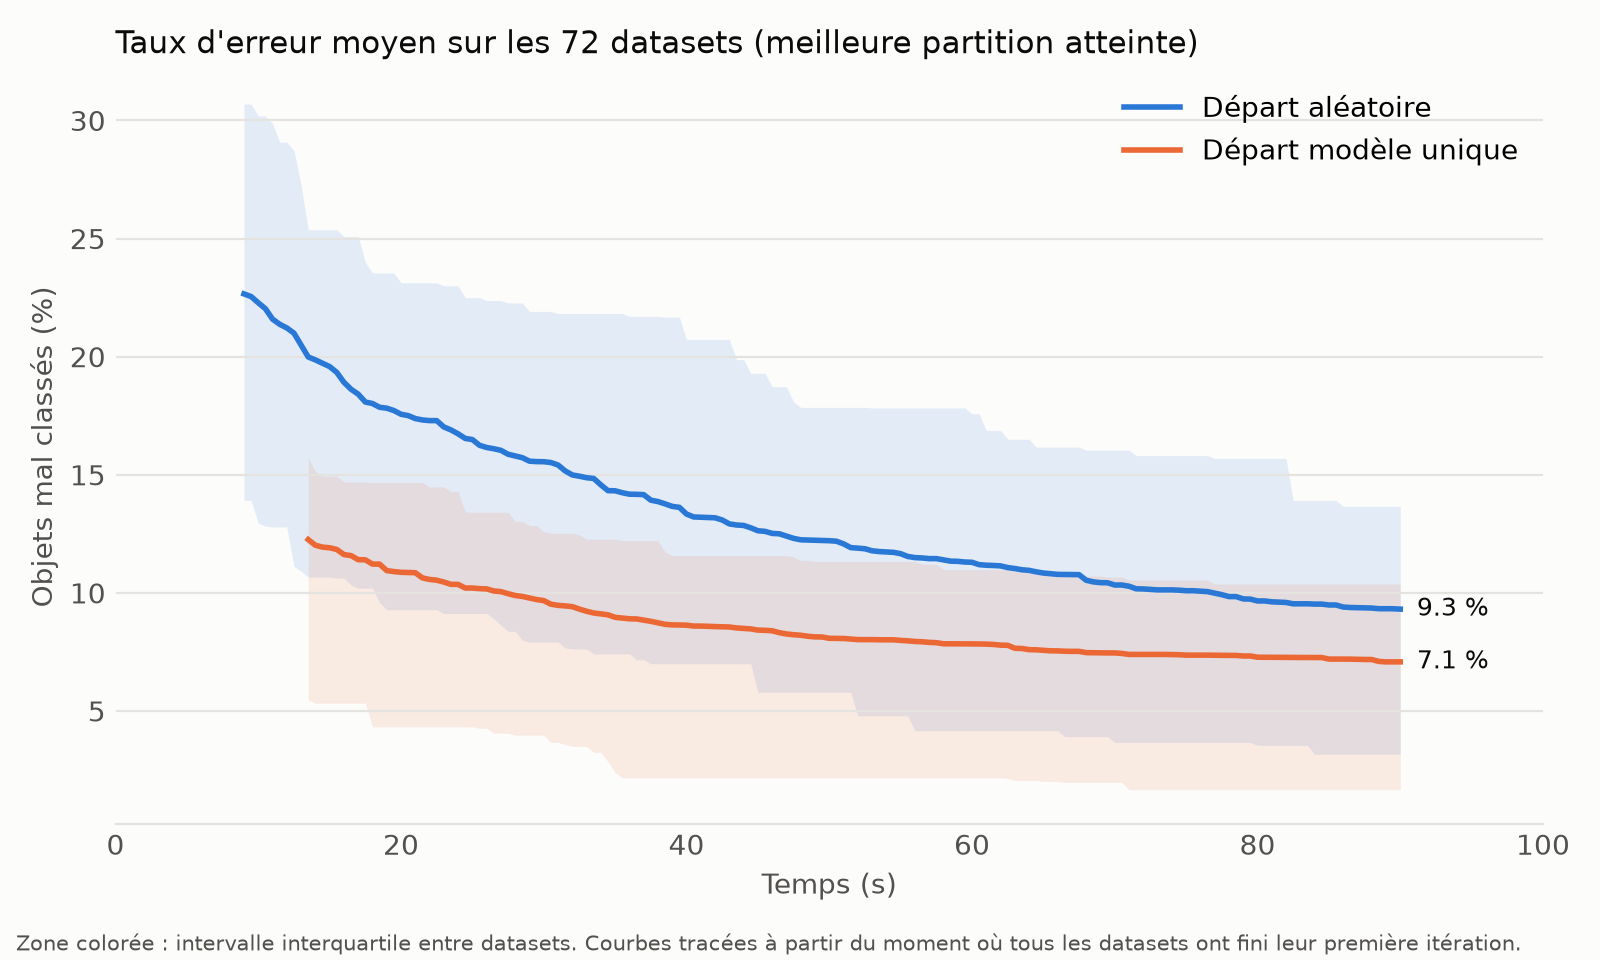
\includegraphics[width=0.78\textwidth]{convergence_erreur_moyenne.png}
\caption{Taux d'erreur moyen en fonction du temps sur les 72 datasets.}
\label{fig:global}
\end{figure}

\subsection{Les datasets de type B sont plus difficiles}

Comme attendu, les datasets de type B sont plus difficiles que ceux de type A (figure~\ref{fig:types}) : les
deux méthodes y partent de plus haut et finissent avec 2,5 à 3,5 points d'erreur de plus. Le classement des
méthodes est le même dans les deux cas, et l'avantage du départ modèle unique est même plus marqué sur le
type B.

\begin{figure}[h]
\centering
\begin{subfigure}{0.49\textwidth}
  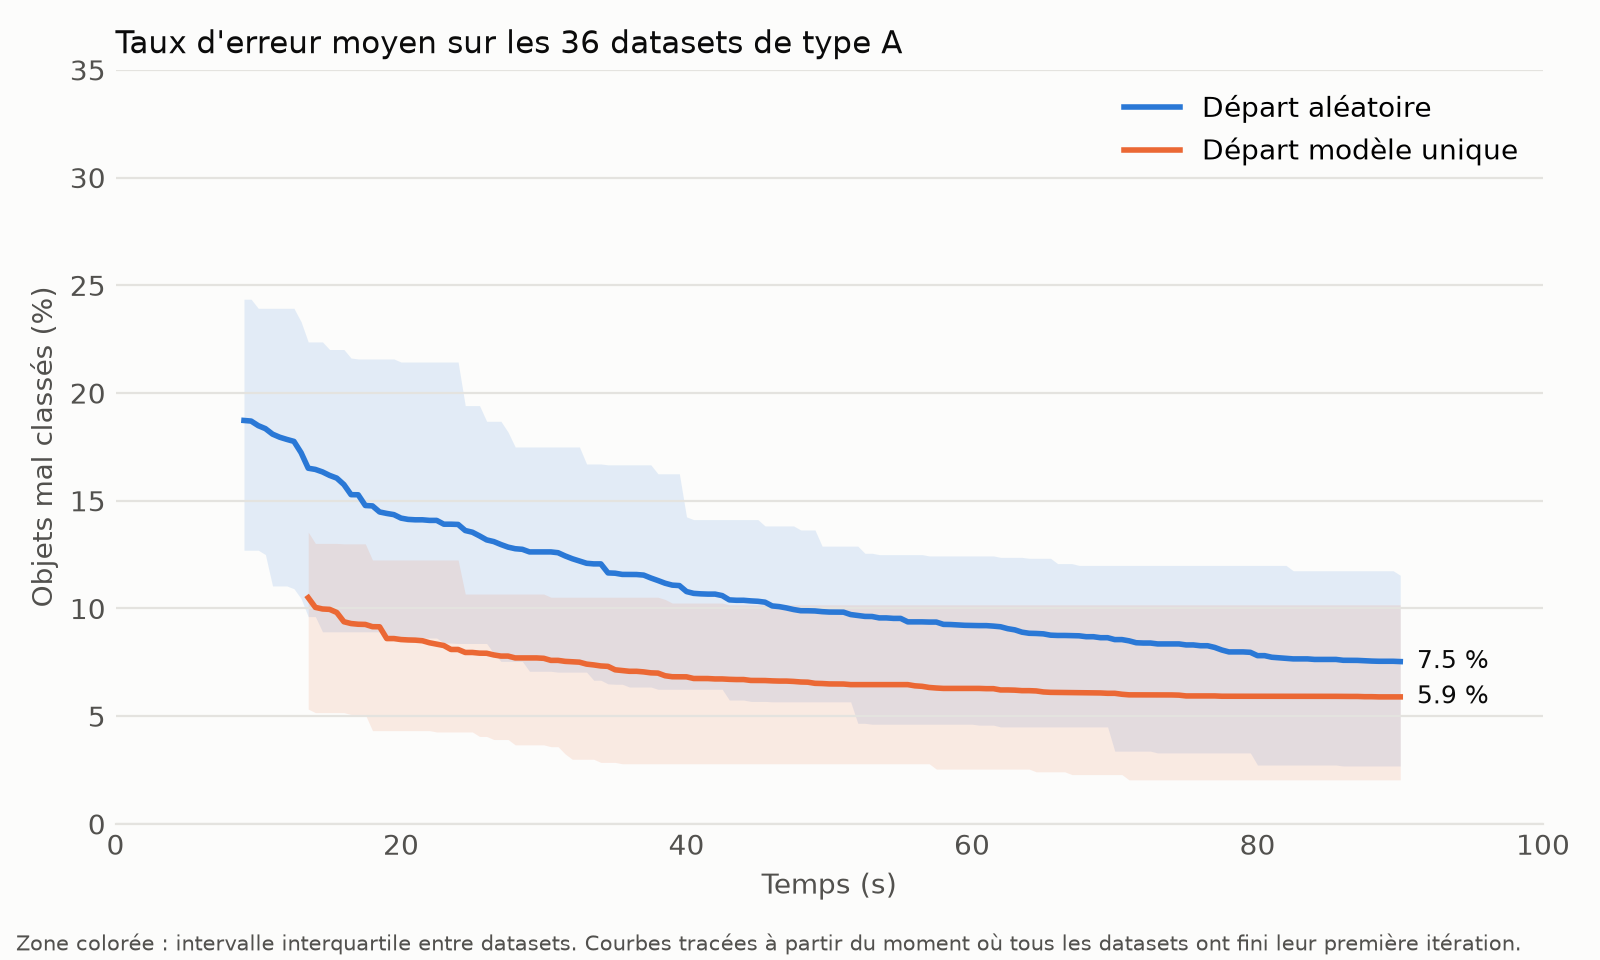
\includegraphics[width=\textwidth]{convergence_type_a.png}
  \caption{Type A : 7,5\,\% (aléatoire) contre 5,9\,\%.}
\end{subfigure}
\hfill
\begin{subfigure}{0.49\textwidth}
  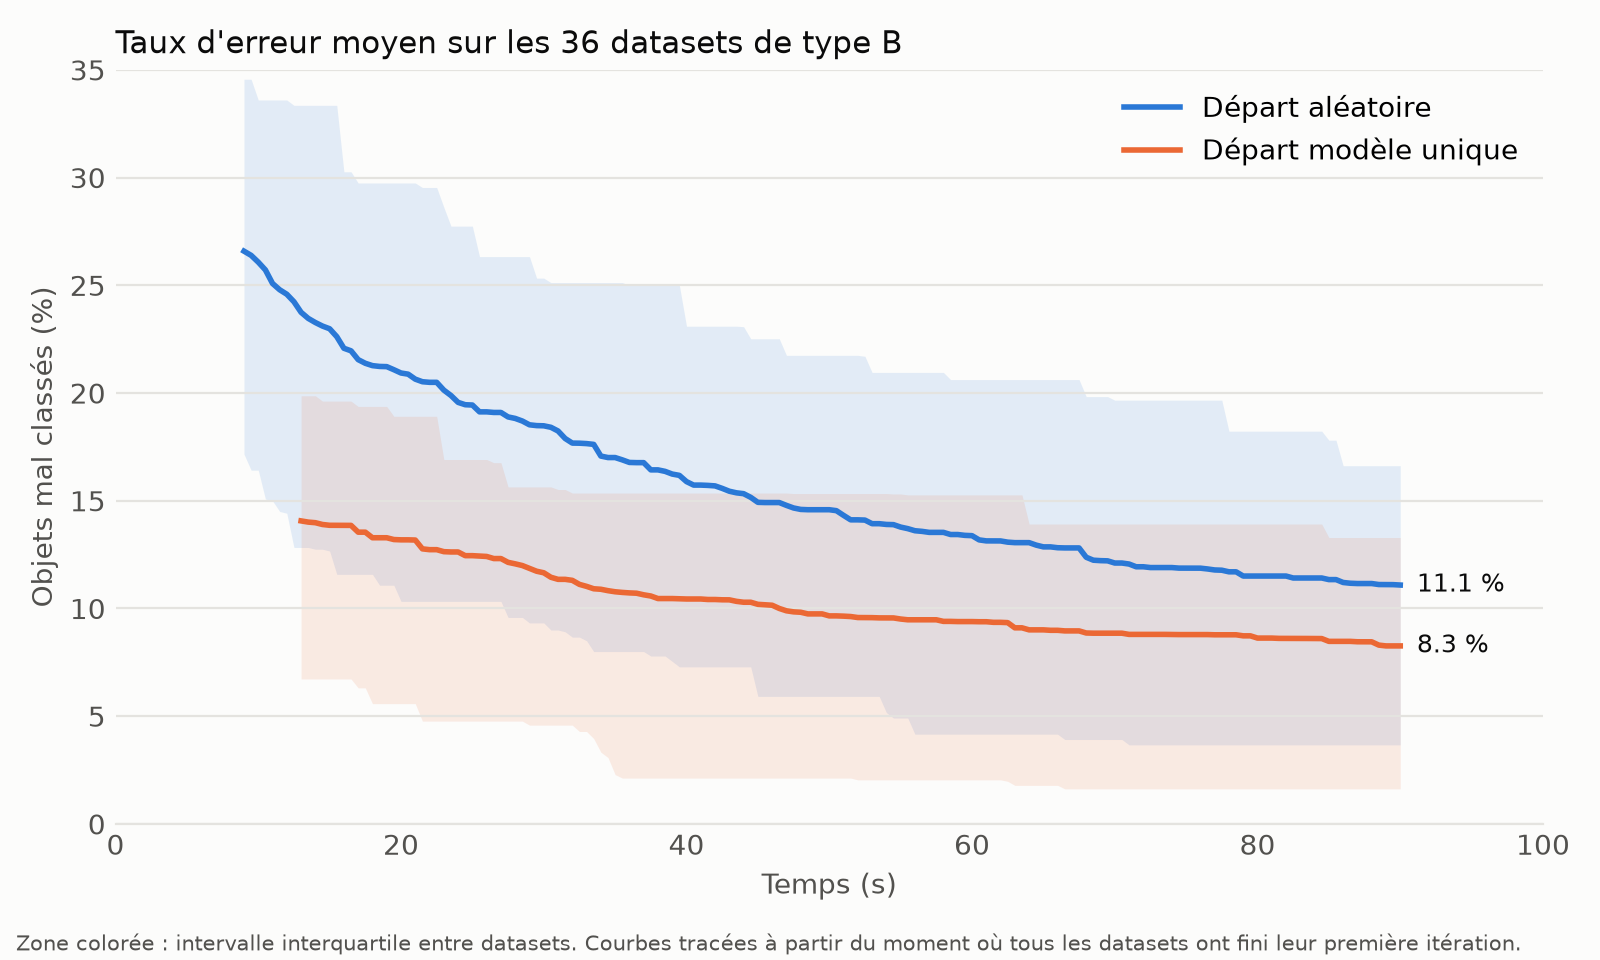
\includegraphics[width=\textwidth]{convergence_type_b.png}
  \caption{Type B : 11,1\,\% (aléatoire) contre 8,3\,\%.}
\end{subfigure}
\caption{Taux d'erreur moyen selon le type de dataset (même échelle).}
\label{fig:types}
\end{figure}

\subsection{Une erreur irréductible due au bruit}

La moitié des datasets comporte 10\,\% d'affectations bruitées, qu'aucun couple de modèles ne devrait pouvoir
expliquer. Sur l'ensemble des 72 datasets, on s'attend donc à une erreur \emph{irréductible} d'environ
$0{,}5\times 0\,\% + 0{,}5\times 10\,\% = 5\,\%$ : avec un taux d'erreur total de 7,0\,\%, l'erreur imputable à
notre méthode n'est que de l'ordre de 2 points. La figure~\ref{fig:bruit} sépare les deux cas : sans bruit, le
départ modèle unique atteint 3,0\,\% d'erreur (contre 5,4\,\% pour le départ aléatoire) ; avec 10\,\% de bruit,
il finit à 11,1\,\%, soit environ 1 point au-dessus du plancher.

L'écart entre datasets bruités et non bruités (8,1 points) est cependant inférieur aux 10 points attendus, et
certaines exécutions descendent sous la ligne des 10\,\% (jusqu'à 3,7\,\% sur un dataset). Cela s'explique en
partie par le hasard, mais aussi probablement par un léger \textbf{surapprentissage du bruit}, de l'ordre de 1 à
2\,\% : avec deux modèles, un objet dont la catégorie a été modifiée par le bruit peut être correctement expliqué
par l'\emph{autre} modèle, et l'heuristique le place alors dans l'autre segment.

\begin{figure}[h]
\centering
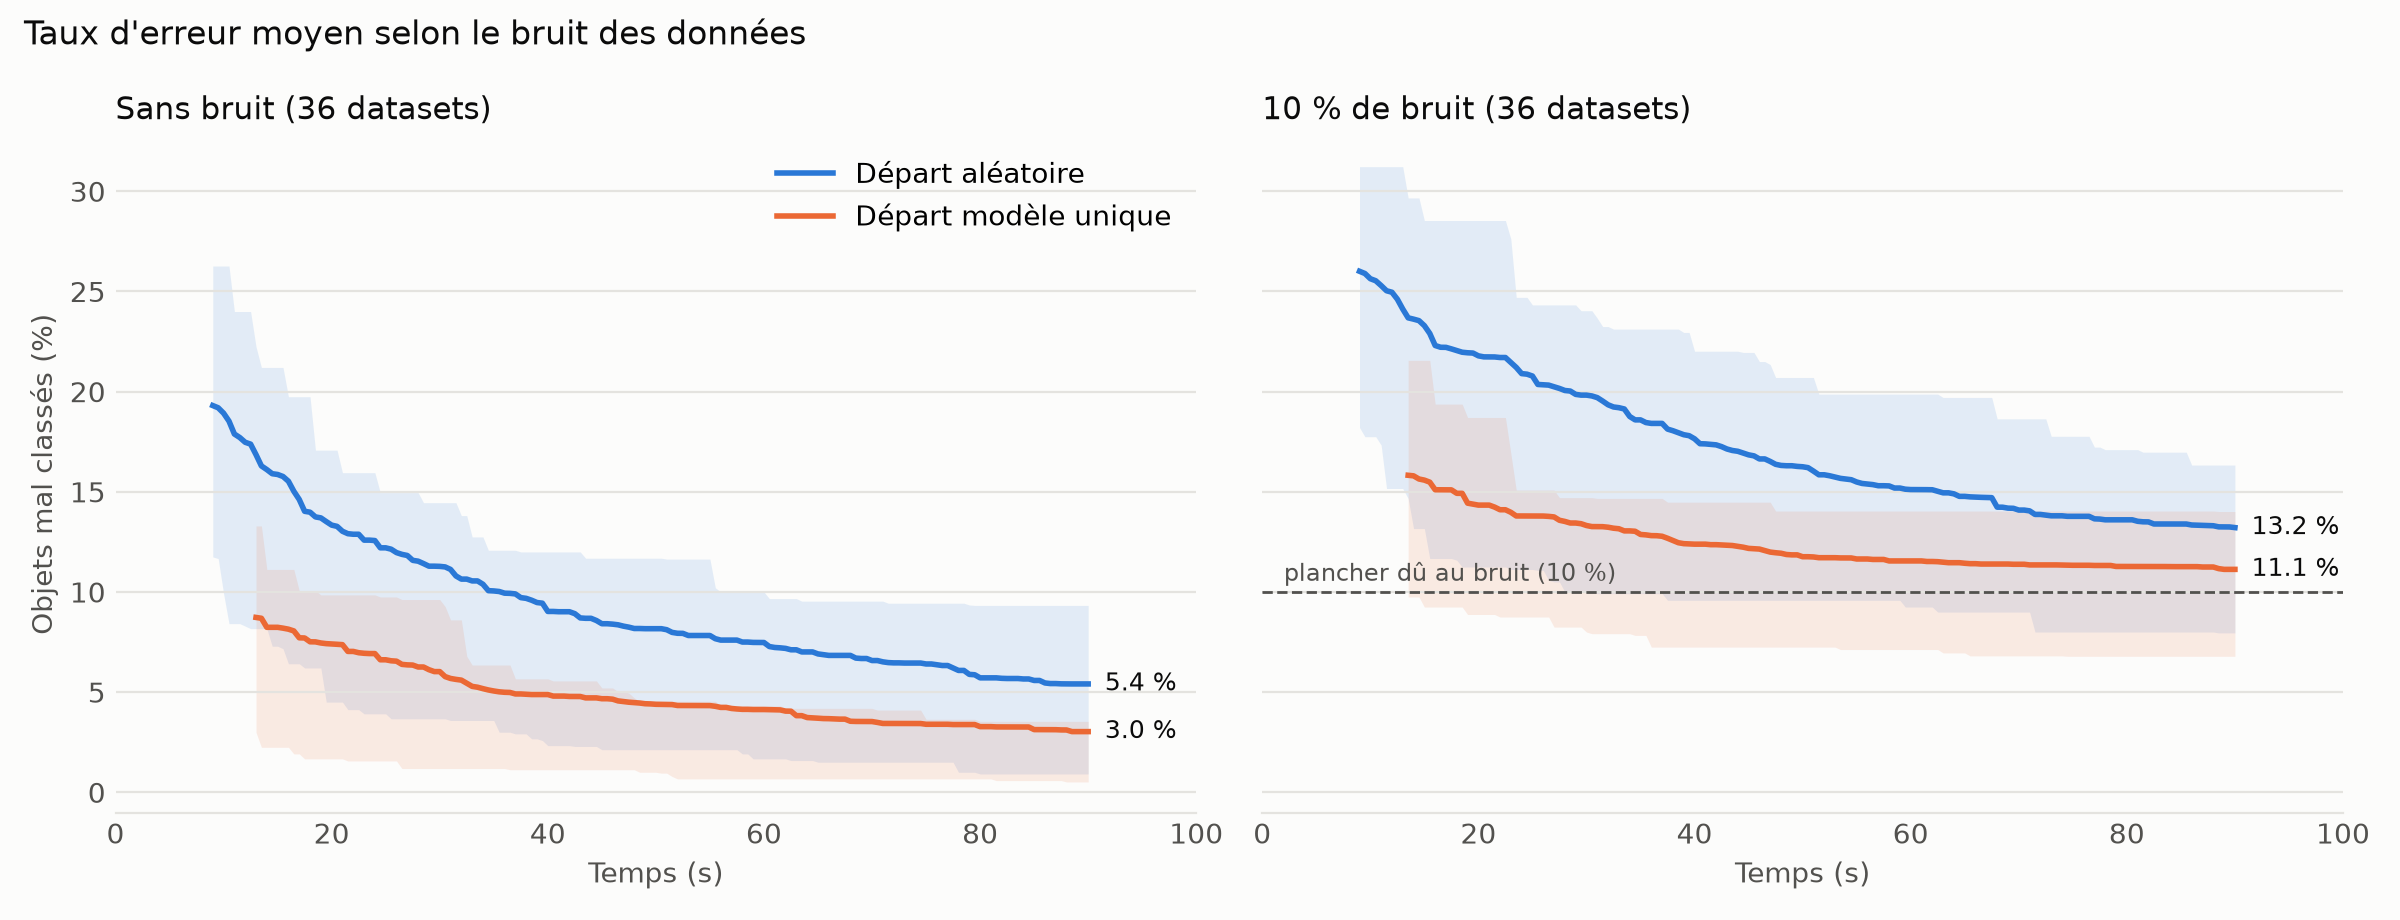
\includegraphics[width=\textwidth]{convergence_par_bruit.png}
\caption{Taux d'erreur moyen sans bruit et avec 10\,\% de bruit (ligne pointillée : plancher dû au bruit).}
\label{fig:bruit}
\end{figure}

\subsection{Un avantage encore plus net sur les segments déséquilibrés}

Comme attendu, le départ modèle unique est encore plus efficace quand les segments sont déséquilibrés
(figure~\ref{fig:repartition}). En 75/25, le modèle unique apprend surtout le segment majoritaire, et ses erreurs
désignent bien le segment minoritaire : la partition de départ ne contient en moyenne qu'environ 10\,\% d'erreur
(6,4\,\% seulement sur les datasets sans bruit), contre 20\,\% pour le départ aléatoire. Il converge alors en 30 à
40\,s et finit à 6,1\,\% d'erreur, contre 8,9\,\% (2,3\,\% contre 5,2\,\% sans bruit). En 50/50, le modèle unique est
un compromis entre les deux comportements et son avantage se réduit (8,0\,\% contre 9,7\,\%).

\begin{figure}[h]
\centering
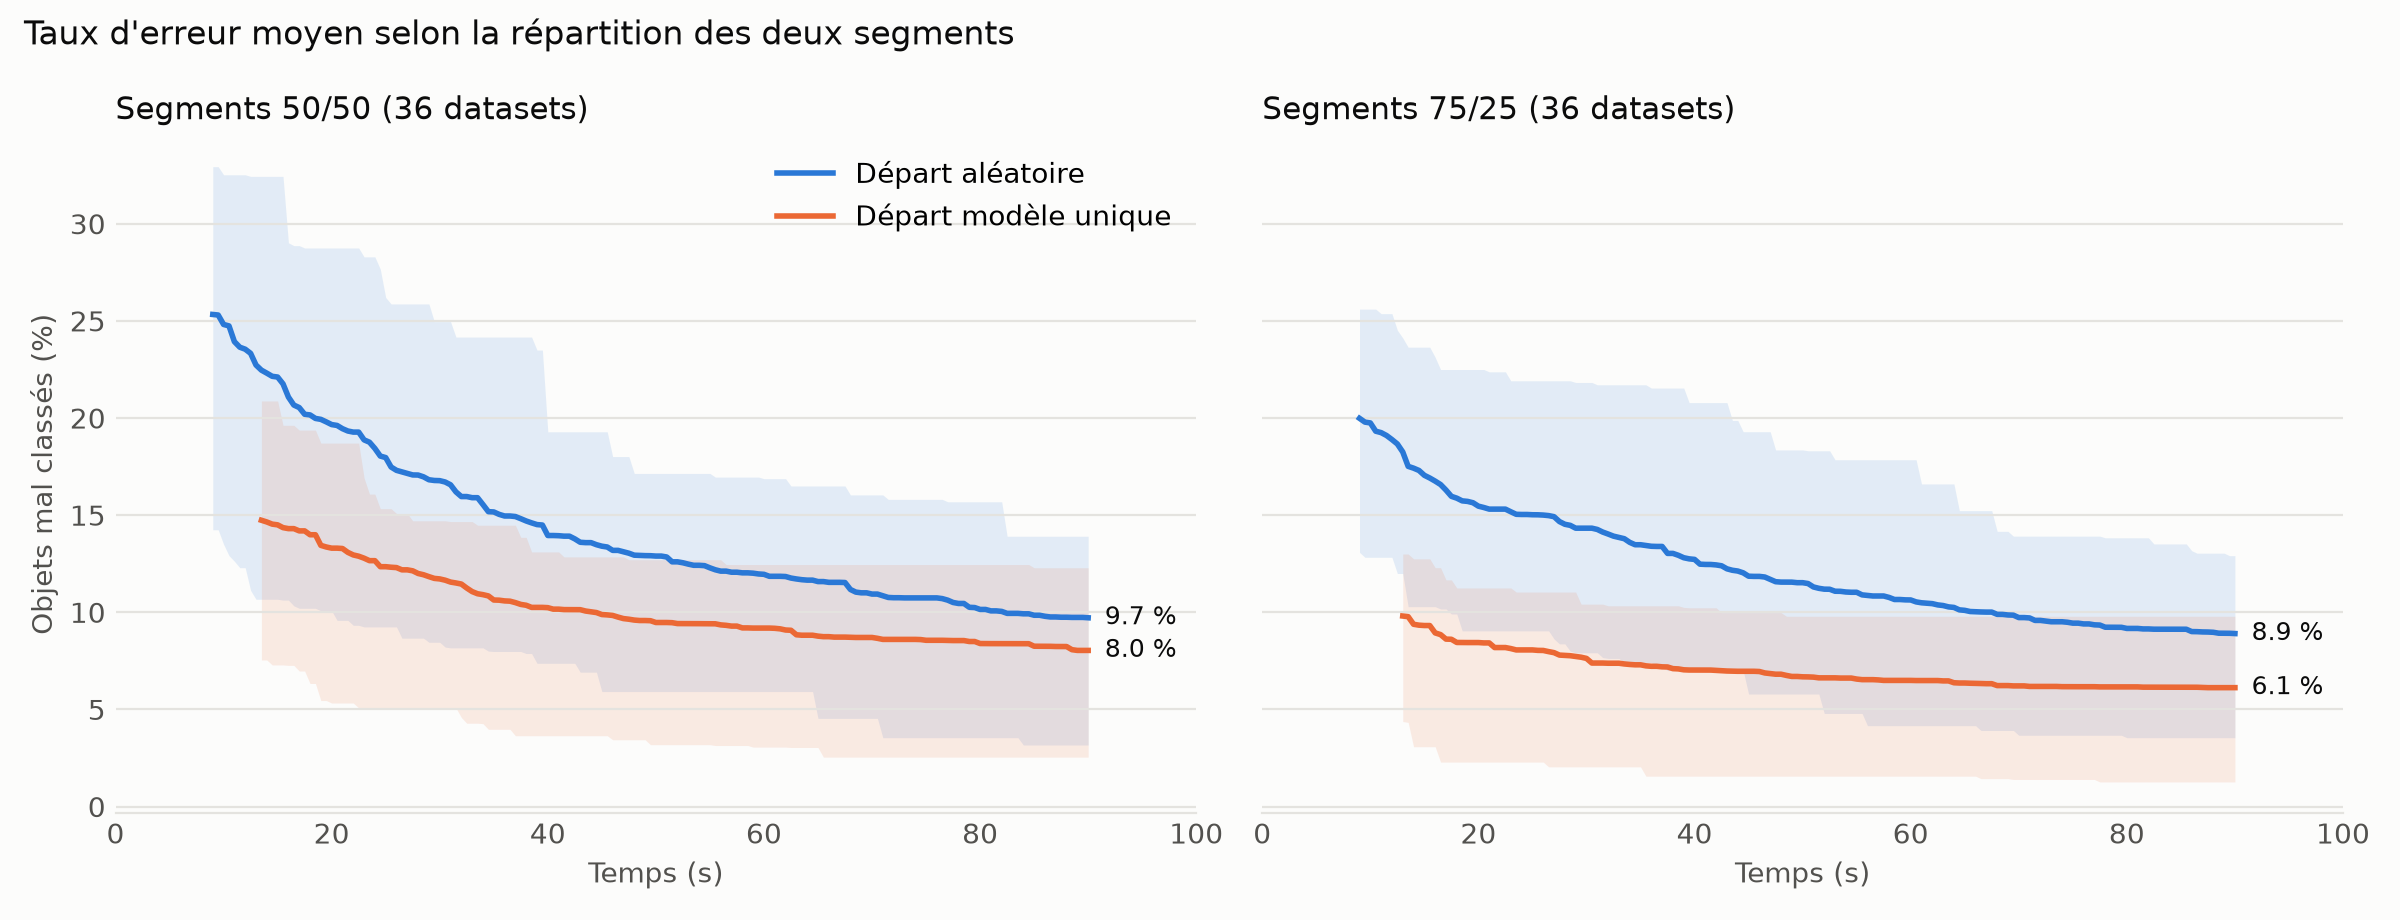
\includegraphics[width=\textwidth]{convergence_par_repartition.png}
\caption{Taux d'erreur moyen selon la répartition des segments.}
\label{fig:repartition}
\end{figure}

Enfin, la difficulté augmente avec la taille du learning set et du problème : sur les datasets de 1\,200 objets,
le départ aléatoire n'a pas convergé en 90\,s (13,0\,\% d'erreur contre 9,2\,\% pour le départ modèle unique,
figure~\ref{fig:taille}), car chaque apprentissage y est plus long et le budget permet moins d'itérations.

\begin{figure}[h]
\centering
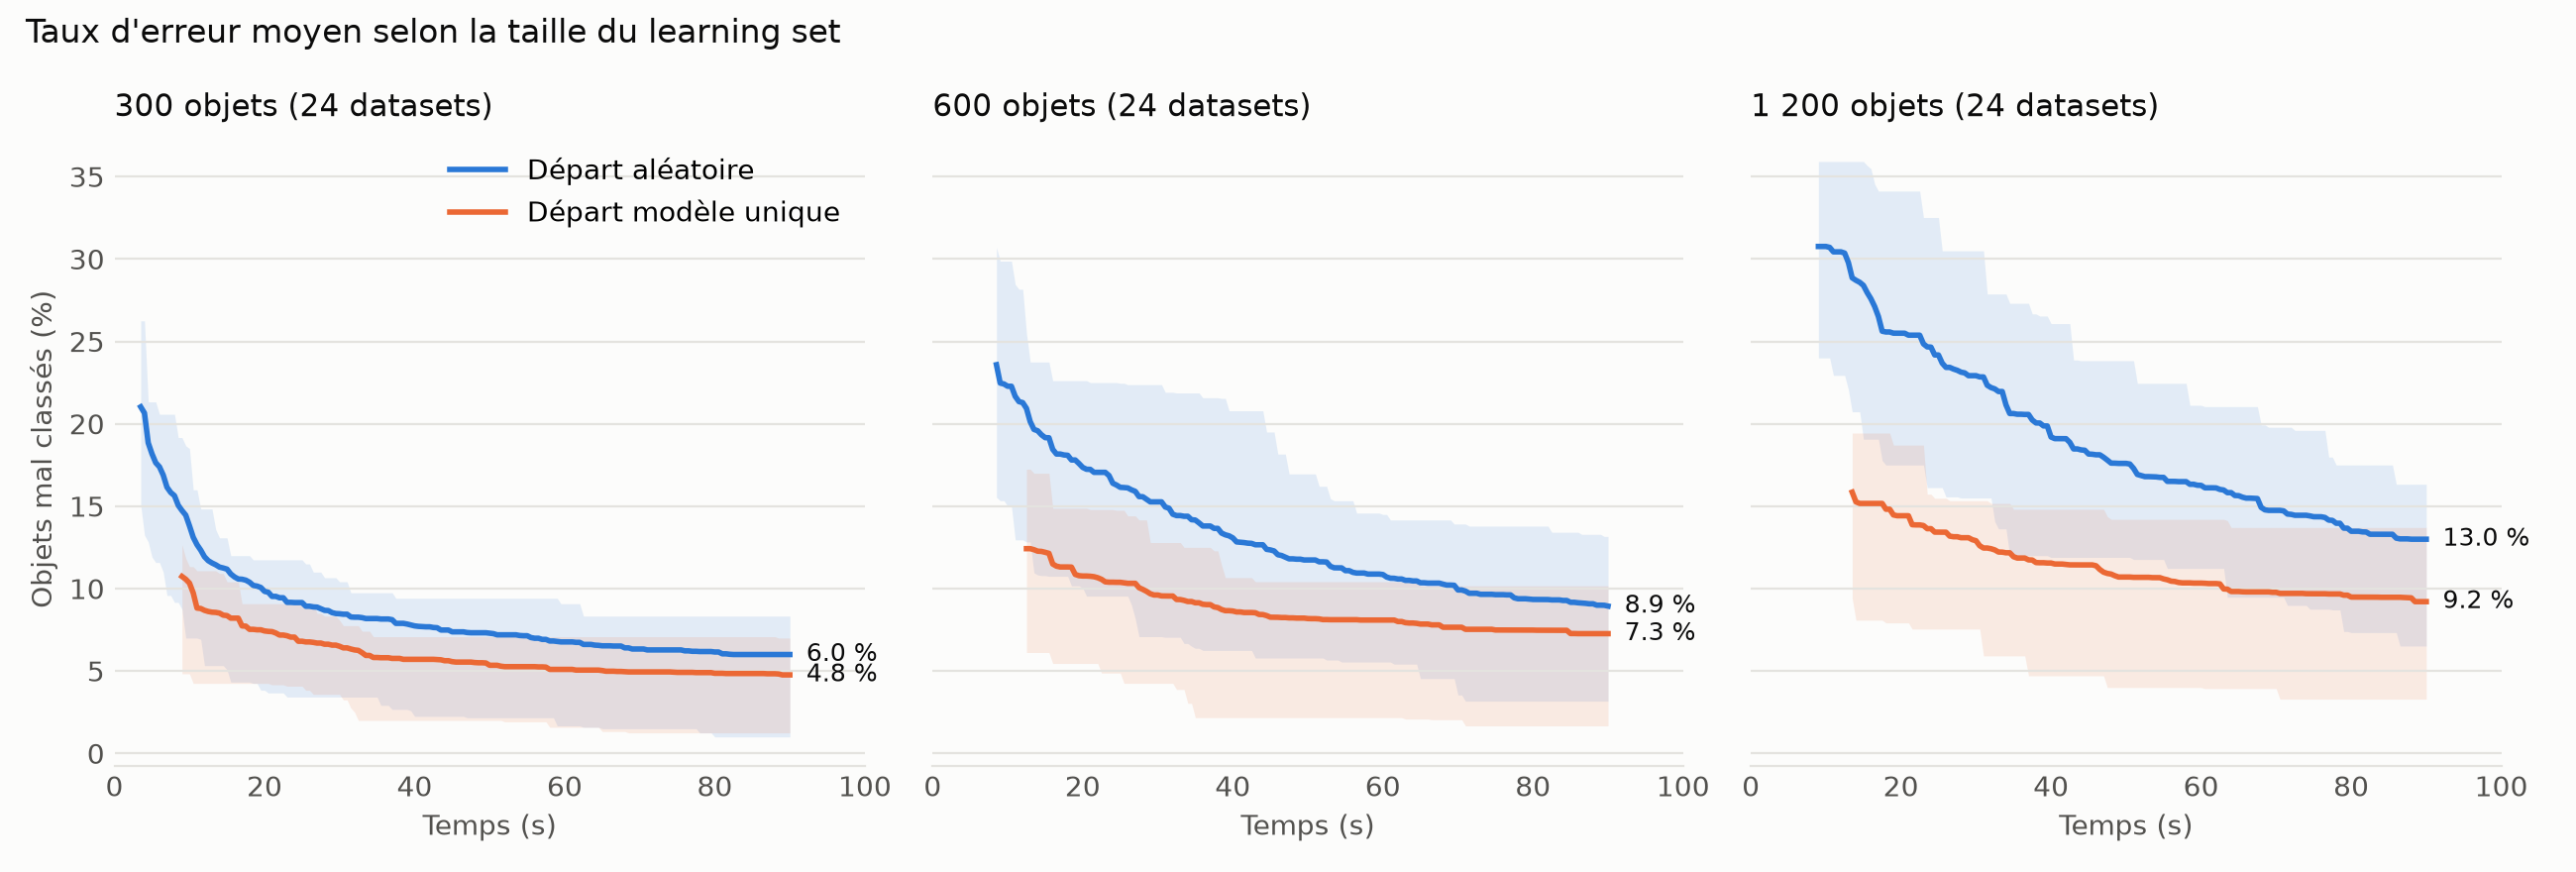
\includegraphics[width=\textwidth]{convergence_par_taille.png}
\caption{Taux d'erreur moyen selon la taille du learning set.}
\label{fig:taille}
\end{figure}

% =====================================================================
\section{Validation empirique sur données synthétiques}

Sur les datasets fournis, le segment de chaque objet est inconnu : un faible taux d'erreur montre que deux
modèles \emph{expliquent} bien les données, mais pas qu'ils sont les \emph{vrais} modèles. Pour le vérifier, nous
générons deux modèles MR-Sort $M_1'$ et $M_2'$ (tirés comme dans Leroy, Mousseau et Pirlot, 2011), des objets
uniformes dans $[0,1]^n$ répartis aléatoirement entre les deux segments, et classons chaque objet avec le
modèle de son segment. Nous lançons ensuite les deux heuristiques (90\,s chacune) sur ce learning set.

Comme vu au jalon 1 (question iii), deux modèles MR-Sort aux paramètres différents peuvent prendre exactement
les mêmes décisions : comparer les poids, seuils ou profils appris à ceux de $M_1'$ et $M_2'$ n'aurait pas de
sens. La validation est donc \textbf{empirique}, fondée uniquement sur les décisions :
\begin{itemize}
  \item \textbf{accord des modèles} : sur un ensemble de test de 10\,000 objets nouveaux, proportion d'objets
        affectés à la même catégorie par $M_j'$ et par le modèle appris $M_j^*$ ;
  \item \textbf{partition retrouvée} : proportion d'objets du learning set remis dans leur vrai segment, en
        prenant la meilleure des deux numérotations (les étiquettes des segments sont interchangeables). Nous
        la mesurons sur les seuls \emph{objets discriminants}, que $M_1'$ et $M_2'$ classent différemment :
        un objet que les deux vrais modèles classent dans la même catégorie peut être placé dans l'un ou
        l'autre segment sans erreur, et ne permet pas de juger.
\end{itemize}

\begin{table}[h]
\centering
\small
\setlength{\tabcolsep}{4pt}
\begin{tabularx}{\textwidth}{lllCCCC}
\toprule
Configuration & Seg. & Départ & Erreur (appr.) & Bon segment (discr.) & Accord $M_1'/M_1^*$ & Accord $M_2'/M_2^*$ \\
\midrule
$n=6$, $p=3$, 300 obj. & 50/50 & aléatoire     & 1,0\,\% & 79,4\,\% & 68,2\,\% & 76,8\,\% \\
                       &       & modèle unique & 0,8\,\% & \textbf{81,5\,\%} & \textbf{76,9\,\%} & \textbf{82,0\,\%} \\
\addlinespace
$n=6$, $p=3$, 600 obj. & 50/50 & aléatoire     & 0,3\,\% & \textbf{82,3\,\%} & \textbf{73,2\,\%} & \textbf{79,6\,\%} \\
                       &       & modèle unique & 2,9\,\% & 68,5\,\% & 68,2\,\% & 77,9\,\% \\
\addlinespace
$n=6$, $p=3$, 600 obj. & 75/25 & aléatoire     & 1,7\,\% & 71,4\,\% & 71,5\,\% & 76,3\,\% \\
                       &       & modèle unique & 0,9\,\% & \textbf{90,2\,\%} & \textbf{92,2\,\%} & \textbf{81,1\,\%} \\
\addlinespace
$n=8$, $p=4$, 600 obj. & 50/50 & aléatoire     & 4,7\,\% & \textbf{86,4\,\%} & \textbf{82,2\,\%} & \textbf{80,3\,\%} \\
                       &       & modèle unique & 7,4\,\% & 78,8\,\% & 70,8\,\% & 69,6\,\% \\
\bottomrule
\end{tabularx}
\caption{Validation sur données synthétiques sans bruit (moyenne de 3 essais par configuration, mêmes données
pour les deux départs).}
\label{tab:validation}
\end{table}

Le tableau~\ref{tab:validation} conduit à trois constats :
\begin{itemize}
  \item \textbf{Bien expliquer les données ne suffit pas à retrouver les vrais modèles.} Les deux heuristiques
        expliquent presque parfaitement le learning set (1 à 7\,\% d'erreur), mais l'accord avec les vrais
        modèles n'est que de 68 à 92\,\%, et 69 à 90\,\% des objets discriminants sont remis dans leur vrai
        segment. Avec deux modèles, beaucoup de couples (partition, modèles) différents expliquent les mêmes
        données : c'est l'équivalent, pour deux segments, de la non-unicité des paramètres vue au jalon 1.
  \item \textbf{Le départ modèle unique est nettement meilleur sur les segments déséquilibrés} : en 75/25, il
        retrouve 90\,\% des objets discriminants (contre 71\,\%) et un modèle majoritaire en accord à 92\,\% avec
        le vrai (contre 72\,\%). Cela confirme l'intuition de la méthode : le modèle unique apprend d'abord le
        segment majoritaire.
  \item \textbf{En 50/50, aucune méthode ne domine} : le départ modèle unique l'emporte sur la configuration à
        300 objets, le départ aléatoire sur les deux configurations à 600 objets. Le modèle unique est alors un
        compromis entre les deux comportements, et son point de départ est moins informatif. Avec seulement
        3 essais par configuration, ces écarts de quelques points ne sont pas significatifs.
\end{itemize}

% =====================================================================
\section{Conclusion et limites}

L'heuristique d'alternance partition / apprentissage, avec \texttt{lincs} pour apprendre chaque modèle, réduit
l'erreur d'un modèle unique de 32\,\% à 7\,\% en 90\,s, dont environ 5 points sont dus au bruit des données.
Initialiser la partition à partir d'un modèle MR-Sort unique donne un bien meilleur point de départ, une
convergence plus rapide et une erreur finale plus faible que le départ aléatoire, en particulier sur les
datasets difficiles (type B, 1\,200 objets) et déséquilibrés. La validation sur données synthétiques confirme
cet avantage sur les segments déséquilibrés, où le départ modèle unique retrouve nettement mieux les vrais
segments et les vrais modèles.

Trois limites sont à garder en tête :
\begin{itemize}
  \item le taux d'erreur est mesuré sur les objets d'apprentissage : la validation synthétique montre que deux
        modèles peuvent expliquer presque parfaitement les données sans coïncider avec les vrais modèles (accord
        de 68 à 92\,\%). Les modèles appris sont des explications plausibles des données, pas nécessairement
        les comportements réels des deux segments ;
  \item la validation ne compte que 3 essais par configuration : elle suffit à montrer l'avantage du départ
        modèle unique en 75/25, mais pas à départager les deux méthodes en 50/50 ;
  \item le résultat dépend un peu de la charge de la machine, puisque chaque apprentissage \texttt{lincs} est
        limité en temps.
\end{itemize}

\end{document}
